\documentclass[11pt,a4paper]{article}

%\input{symbols.tex}
\usepackage{amssymb}
\usepackage{german}
\usepackage{rawfonts}
\usepackage[dvips]{epsfig}
%\usepackage[dvips]{graphicx}
%\usepackage[pdftex]{graphicx}
\sloppy
\parindent0em
\parskip0.2em
%\topmargin-1.3 cm
%\textheight26cm
%\textwidth16.8cm
%%\oddsidemargin-0.5cm
%\oddsidemargin-1.5cm

\pagestyle{empty}

%\include{prepictex}
%\include{pictex}
%\include{postpictex}

\font \sfbold=cmssbx10

\input{almS}

\begin{document}

%\head{1}{}

\setcounter{section}{1}

%\setcounter{aufg}{0}

%\rule{\textwidth}{0.03cm}
%\parskip0.6cm

\textbf{ISDS Individual Assignment 1 Solutions}


\vspace{0.2cm}

\begin{question}
Multiple choice questions. \textcolor{blue}{\textbf{[1 mark]} per correct answer}
\begin{enumerate}
\item A short e-survey is released, asking the following question: ``How many cups of tea do you drink a day?''. The available answers were ``0'', ``1'', ``2``, and ``3 or more''.

What type of data is the e-survey collecting?

\begin{enumerate}
\item Nominal
\item \textcolor{blue}{Ordinal}
\item Discrete
\item Continuous
\end{enumerate}




\item Data is collected relating to the continent of origin of students at Durham. The data is to be shown graphically to the University Council, to help them understand where students come from most often, and least often.

Council will want to compare numbers between continents - they are not interested in the proportion each continent of origin makes up of the whole of the student body. Which of the following graphs would be the best method for displying this data?

\begin{enumerate}
\item \textcolor{blue}{Bar chart}
\item Pie chart
\item Histogram
\item Stem and leaf diagram
\end{enumerate}



\item In a recent survey, 46\% of the British population said they preferred dogs to cats. In another recent survey, 12\% of the Britih population listed jazz as one of their favourite musical genres.

Assume that whether a person prefers dogs to cats is independent of whether they consider jazz one of their favourite musical genres. What probability, expressed as a percentage, should we give to the event that a British person prefers dogs to cats \textbf{and} considers jazz one of their favourite musical genres.
\begin{enumerate}
\item $58\%$
\item \textcolor{blue}{$5.52\%$}
\item $55.2\%$
\item $5.80\%$
\end{enumerate}
\textcolor{blue}{The two important ideas here are i) the proportion of people in the population who have a given quality is equivalent to the probability that a \textbf{specific} person from that population has the given quality, and ii) we are allowed to assume these qualities are independent. We can therefore use the multiplicative rule - multiplying the  probabilities of each separate quality together to get the probability someone has both qualities}

\item Consider an outcome space $\Omega=\{1,8,15,35,69,732,983\}$. Let $A=\{1,8,69,983\}$ and let $B=\{1,8,15,35,69\}$.

Assuming a uniform probability distribution on $\Omega$, which of these is the probability that $A$ AND $B$ occur?

\begin{enumerate}
\item \textcolor{blue}{$\frac{3}{7}$}
\item $\frac{4}{7}$
\item $\frac{5}{7}$
\item $\frac{6}{7}$
\end{enumerate}

\textcolor{blue}{There are four outcomes in $A$, and five in $B$, but only three outcomes in both $A$ \textbf{and} $B$. The probability of getting an outcome that is in $A$ \textbf{and} in $B$ is therefore $\frac{3}{7}$.}

\item A random variable U is defined with the probability density function below:
\begin{eqnarray*}
f(u)=\begin{cases} 
      \frac{u}{2} & 0\leq u \leq 2 \\
      0 & \text{otherwise}
   \end{cases}.
\end{eqnarray*}

Which of the following is the value of $P(U>0.30)$?

\begin{enumerate}
\item $0.09775$
\item $0.03$
\item $0.70$
\item \textcolor{blue}{$0.9775$}
\end{enumerate}

\textcolor{blue}{We have}

\textcolor{blue}{
\begin{eqnarray*}
P(U>0.30)&=&\int_{0.3}^{\infty}f(u)du\\
&=& \int_{0.3}^{2}\frac{u}{2}du
\end{eqnarray*}
}
\textcolor{blue}{using the fact that the integral of 0 is always 0, so we don't need to worry about the part of the integral where $f(u)=0$.}

\textcolor{blue}{Next,}

\textcolor{blue}{
\begin{eqnarray*}
\int_{0.3}^{2}\frac{u}{2}du &=&\left[\frac{u^2}{4}\right]^2_{0.3}\\
&=&\frac{4}{4}-\frac{0.09}{4}\\
&=&0.9775.
\end{eqnarray*}
}


\end{enumerate}



\end{question}



\begin{question}
Using the \texttt{ToothGrowth} data set in \texttt{R}:
\begin{enumerate}
\item Find the modal tooth length across the entire data set.

\textcolor{blue}{26.4 \textbf{[1 mark]}}
\item Find the mean tooth length for guinea pigs who were given their vitamins via orange juice.



\textcolor{blue}{20.66 \textbf{[1 mark]}}

\item Create a diagram in \texttt{R} of two box-and-whisker plots, one showing tooth length for guinea pigs given their vitamins via asorbic acid, and one showing tooth length for guinea pigs given their vitamins via orange juice. The box-and-whisker plots should be adjacent to each other, using the same axis, to enable easy comparison.

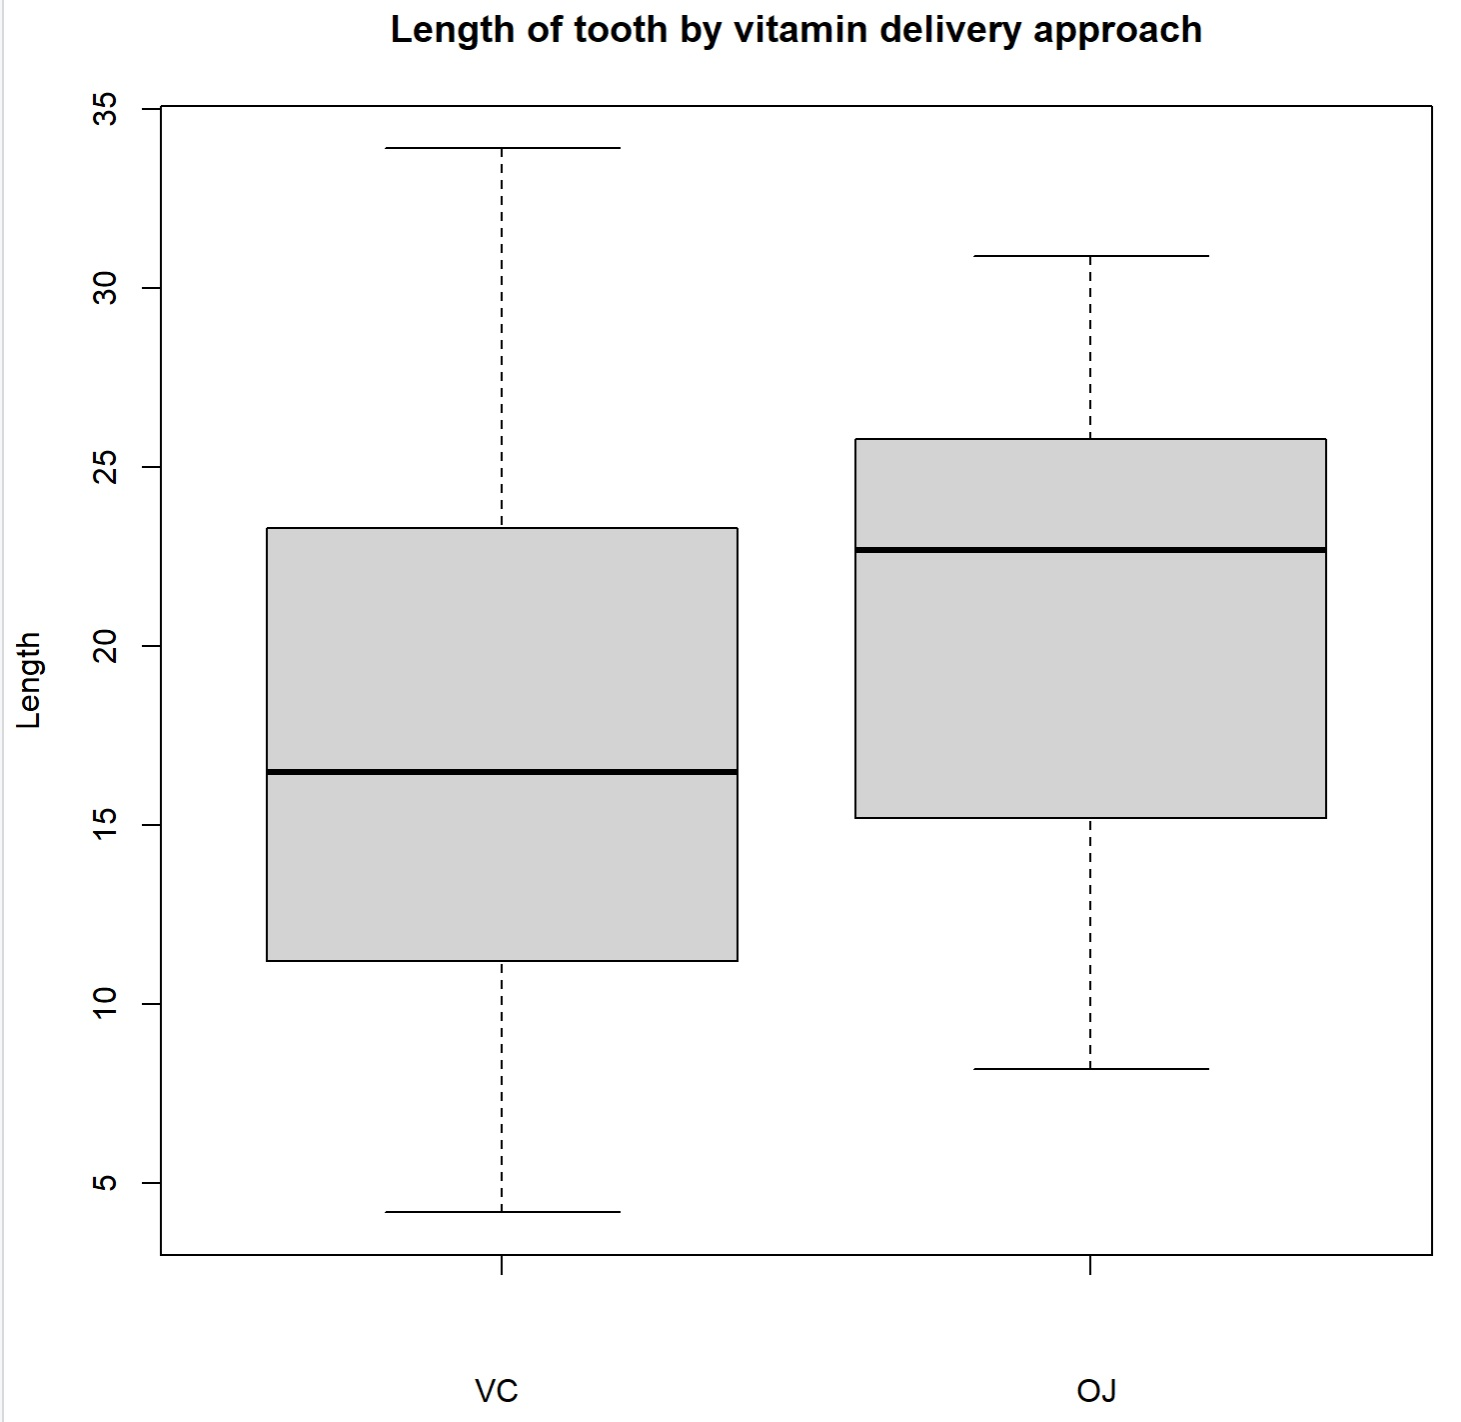
\includegraphics[scale=6]{ISDSA1p1.jpg}

\textcolor{blue}{\textbf{[2 marks]}}

\item Using the box-and-whisker plots created in Question 1.2.3, comment on which of the two vitamin delivery approaches is more effective in promoting tooth growth. Justify your answer.

\textcolor{blue}{OJ is both a more reliable approach to vitamin dissemination (smaller IQR) and with a higher median. This would suggest OJ is the superior option. On the other hand, the maximum length was achieved via VC. \textbf{[2 marks] for similar comments, or other valid comments.}}

\end{enumerate}

\end{question}

\begin{question}
A company that produces party poppers claims on their website that only 0.6\% of their party poppers will fail to go off when the string is pulled.
\begin{enumerate}
\item The company sells party poppers in boxes of 200. What is the expected number of party poppers in a box which will fail to go off?
\textcolor{blue}{
\begin{eqnarray*}
0.006\times 200=1.2
\end{eqnarray*}
}
\textcolor{blue}{\textbf{[1 mark]}}

\item I decide I want to represent the number of party poppers which fail to go off in a box using a random variable, $X$.
\begin{enumerate}
\item Which distribution would be the most appropriate to use for $X$? Give both the name of the distribution, and the value of the parameters assuming the company's claim on their website is correct.
\textcolor{blue}{
\begin{eqnarray*}
X\sim Bin(200,0.006)
\end{eqnarray*}
}
\textcolor{blue}{\textbf{[1 mark]}}
\item What assumptions regarding the party poppers would need to hold in order to justify that choice of distribution?

\textcolor{blue}{
Assumptions: a party popper goes off or it doesn't, each party popper goes off or doesn't independently, each party popper has same probability of not going off, the number of poppers in a box is indeed 200
}

\textcolor{blue}{\textbf{[2 marks] for any three of these}}


\end{enumerate}
\item I order a box for myself, but due to an administrative error, the box arrives containing not 200 party poppers, but 2.
\begin{enumerate}
\item Define the distribution for $Y$, the random variable representing the number of party poppers which fail to go off in my box of 2, assuming the claim on the company's website is correct.
\textcolor{blue}{
\begin{eqnarray*}
Y\sim Bin(2,0.006)
\end{eqnarray*}
}
\textcolor{blue}{\textbf{[1 mark]}}

\item Find $E(Y)$ and $\textrm{Var}(Y)$, under the assumptions needed for Question 1.3.2 b), and under the assumption that the claim on the company's website is correct. NOTE: You will need to scan and upload your working.

\textcolor{blue}{We have}

\textcolor{blue}{
\begin{eqnarray*}
E(Y)&=&0\times P(Y=0)+1\times P(Y=1)+2\times P(Y=2)\\
&=& \frac{2!}{1!1!}\times0.006\times(1-0.006)+2\times\frac{2!}{2!0!}\times0.006^2\\
&=&0.0120\\
\textrm{Var}(X)&=&(0-0.012)^2\times P(Y=0)+(1-0.012)^2\times P(Y=1)\\&+&(2-0.012)^2\times P(Y=2)\\
&=&(-0.012)^2\times \frac{2!}{0!2!}\times(1-0.006)^2\\ &+&0.988^2\times\frac{2!}{1!1!}\times0.006\times (1-0.006)+1.988^2\times \frac{2!}{2!0!}\times0.006^2\\
&=&0.0119
\end{eqnarray*}
}

\textcolor{blue}{\textbf{[3 marks]}}

\end{enumerate}
\end{enumerate}



\end{question}



\begin{question}
Let $X\sim Pois(0.4)$, and let $Y\sim Pois(\lambda)$. Find:
\begin{enumerate}
\item $P(X=4)$.

\textcolor{blue}{We have}

\textcolor{blue}{
\begin{eqnarray*}
P(X=4)&=&\frac{e^{-0.4}0.4^4}{4!}\\
&=&0.001
\end{eqnarray*}
}
\textcolor{blue}{\textbf{[1 mark]}}


\item $P(X<3)$. NOTE: You will need to scan and upload your working.

\textcolor{blue}{We have}

\textcolor{blue}{
\begin{eqnarray*}
P(X<3)&=&P(X=0)+P(X=1)+P(X=2)\\
&=&\frac{e^{-0.4}0.4^0}{0!}+\frac{e^{-0.4}0.4^1}{1!}+\frac{e^{-0.4}0.4^2}{2!}\\
&=&0.992
\end{eqnarray*}
}
\textcolor{blue}{\textbf{[2 marks]}}
\item An algebraic expression for $P(Y=4|Y\geq3)$ NOTE: You will need to scan and upload your working.

\textcolor{blue}{We have}

\textcolor{blue}{
\begin{eqnarray*}
P(Y=4|Y\geq3)&=&\frac{P(Y=4\textrm{ AND }Y\geq3)}{P(Y\geq3)}\\
&=&\frac{P(Y=4)}{P(Y\geq3)}\\
&=&\frac{P(Y=4)}{1-P(Y<3)}\\
&=&\frac{\frac{e^{-\lambda}\lambda^4}{4!}}{1-\left(\frac{e^{-\lambda}\lambda^0}{0!}+\frac{e^{-\lambda}\lambda^1}{1!}+\frac{e^{-\lambda}\lambda^2}{2!}\right)}\\
&=&\frac{\lambda^4}{12\left(2e^{\lambda}-2-2\lambda-\lambda^2\right)}
\end{eqnarray*}
}
\textcolor{blue}{\textbf{[3 marks]}}


\end{enumerate}

\end{question}




\end{document}